\chapter{Malware analysis} \label{chap:analysis}
A particular goal of this thesis is to create a dataset of dynamic malware analysis samples. In this chapter, we define the basic notions of malware, PE file and malware analysis. We describe \emph{CAPEv2} sandbox and its output. We also address some cybersecurity challenges and refer to prior arts.

\section{Cybersecurity challenges}
We address the challenges that we find essential, and we refer to the ones listed in \cite{Amit2019}. The authors of that paper also list available datasets for specific kinds of machine learning tasks in cybersecurity.

There are terabytes of data every second in cybersecurity - cloud, IoT, and general network traffic\dots. Supervised machine learning is generally more reliable than unsupervised, so we want these data to be labelled. However, the detection itself has to be fast. The most significant is the ability to detect zero-day attacks and malware variants based on similar attributes. Repeated observations might not be possible because modern malware is flexible. As an example, we can see analysis evasion techniques \cite{Afianian2018}. A significant concern is also bias in the data itself caused by multiple factors - size, noise, sensibility to minor deviations. For instance, if we run several malware samples in a sandbox that has access to the internet and the malware can access its public IP address, the bias might be caused by the geographical location of the edge router. That is something that could ruin our dataset. Another kind of bias is encryption, as mentioned in the thesis introduction.

Regarding the lack of labelled and certainty in the ground truth, we can address several problems. If a human does the labelling process, it becomes slow and subjective. Therefore, the better approach is to develop some heuristics like blacklists, whitelists, or more complex rules/models. The quality of labelling determines the actual performance of our future model and its reliable evaluation. We want to create as general knowledge as possible to face different situations and contexts. Sometimes we cannot gain a sufficient amount of data, e.g. \  \emph{Advanced Persistent Threats} that are disposable and unique attacks. However, unsupervised techniques like anomaly detection or active learning in combination with semisupervised learning might help us.

If we collect the dataset, we should care about its quality. Imbalanced datasets are another problem of cybersecurity. The population of specific attacks is not distributed equally, and even the ratio between benign and malicious varies in time. Another addressed problem is the concept drift. It addresses the decreasing performance of a machine learning model due to the difference in training data and current data (after deployment).  It might be caused by the violated assumptions that we make before the training. That could be solved by a new model or a better ability to adapt existing models in new situations.

\section{Malware}
Malicious code (also called \emph{Malware}) is intended to disrupt a computer, network, or part from functioning. The form or format may vary. It could be a JAVA application, Microsoft office macro or even pdf file. Malware detection, classification and overall research is part of broader branch of \emph{Intrusion detection} \cite{Cole2009}. Attackers use malware to steal data, use target computer (in C2 or DDOS attacks) or even spy on the owner. Malware often gets into the target computer via usual communication channels - emails, USB, web download. \cite{KA2018}. Malware may contain more parts that have a different role, and we call these parts \emph{components}. The software which is not malicious (benign) is often called \emph{cleanware}.

Firstly, let us clarify several terms. \emph{Malware type} denotes a group of malware samples or their components that show the same behaviour. \emph{Malware family} is a collection of malware that has the same code base (uses same code components). An example of such a family might buy \emph{Emotet}, the banking trojan family or CryptoWall, ransomware family. \emph{Malware variant/strain/version} is malware which is in some existing families but includes new parts which were not earlier detected in this family \cite{Cohen2019}.

Based on the specific behaviour, we can distinguish several fundamental types of malware. Each malware sample may have multiple components, and each component may have a different type. The most usual malware types follow (their source is \cite{Cole2009, KA2018, Graham2010, Sikorski2012}).
\begin{itemize}
  \itemsep0em 
  \item \emph{Worm} is malware capable of copying itself in a variety of ways and spreading on multiple devices.
  \item \emph{Virus} is capable of infecting other executable files by injecting its payload. The user then executes the infected files.
  \item \emph{Trojan} disguises itself as a regular program. After installation, they can steal the data, control the target machine\dots
  \item \emph{Backdoor} allow the attacker to access the target machine. The attacker can use multiple machines as a botnet controlled by a command and control server.
  \item \emph{Adware} presents unwanted advertisements to a user of the target machine. They are usually downloaded from the internet.
  \item \emph{Information stealer} aims at the user's data. Examples are sniffers, grabbers, spyware, and key loggers.
  \item \emph{Ransomware} locks users out of their computer or encrypts their data. It usually threatens the user by not decrypting it before they pay some money.
  \item \emph{Rootkit} allow a malware presence concealment.
  \item \emph{Dropper} download malicious code or its updates from the internet. The dropper itself is often harmless.
  \item \emph{Launcher} is responsible for running malicious code, usually stealthy.
\end{itemize}

According to \cite{AVATLASM39:online} the most seen types on Windows operating system are \emph{trojans} and \emph{backdoors}.

\section{File formats}
Malware is defined very generally, and it is not limited to a specific file format. We can find various file types - Portable executable, Portable Document Format, Microsoft office formats, HTML, Archives and many others. According to \cite{AVATLASM39:online} Portable Executable (PE) files are the most seen on Windows machines.

\subsection{Portable Executable}
The portable executable is a file format mainly for executables, object code and data-link libraries (DLLs). It is specific for Windows operation system. For 32-bit, we use the format PE32 and for 64-bit is PE32+. Its complete description is provided by Microsoft \cite{PEFormat89:online}. Description of the essential parts follows.

The PE file includes information necessary for Windows operating system (specifically the dynamic linker) to map the file into memory \cite{Gibert2020}. Usual file extensions are \emph{.exe, .dll, .sys}. It consists of two main parts - \emph{Header} and \emph{Sections} (see \ref{fig:pe}). 

\emph{Header} contains technical details about the executable. The most important parts are:
\begin{itemize}
  \itemsep0em 
  \item DOS header - presented for backward compatibility with older versions of Windows
  \item PE header - executable info such as number of sections, file signature
  \item Optional header - additional info such as the base of data, base of code, address of entry point
  \item Sections table - definition of the loading process
  \item Import/export address table - lookup table (pointers) for imported or exported structures (abbrev. \emph{IAT})
\end{itemize}

\emph{Sections} contains mainly the data and code of the executable file. The most important parts are:
\begin{itemize}
  \itemsep0em 
  \item Code - actual program code (\emph{.text})
  \item Imports/exports - \emph{.idata, .edata}
  \item Data - static constants (\emph{.data}), variables(\emph{.bss}), other resources (\emph{.rsrc}), debug data (\emph{.rdata})
\end{itemize}

The loading process of the PE file starts by parsing and validity checking of the headers and sections table. The file is mapped into memory according to the information in specific header parts. Additional DLLs are loaded into memory based on \emph{IAT}. Finally, the file is executed at a specified entry point. \footnote{source https://github.com/corkami/pics/blob/master/binary/pe101/pe101.png}

\begin{figure}[h]
  \centering
  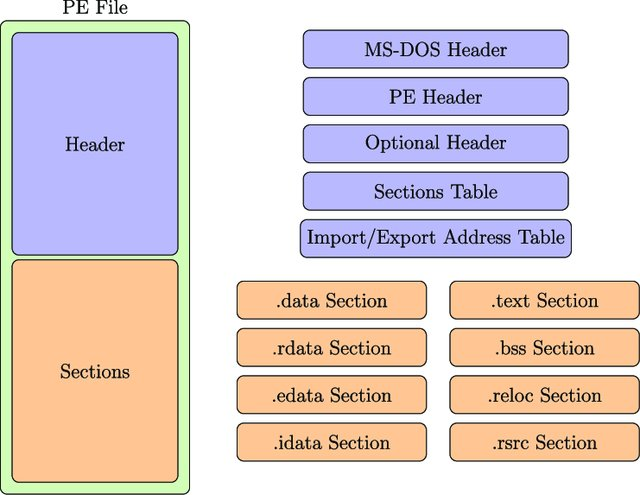
\includegraphics[width=0.8\textwidth]{figures/pe.jpg}
  \caption{PE file structure (source \cite{Gibert2020})}
  \label{fig:pe}
\end{figure}

\section{Malware analysis}
Malware analysis is a process leading to a deeper understanding of malware features, behaviour, and goals. We can use several techniques to analyze a malware sample, and not all of them require its execution.

Malware analysis is the most relevant if we do not have the source code of the malware binary because its examination would often give us much more information. We see the sample as a black box \cite{Sikorski2012}.

The goal of the security threats research and description is to find a proper response - prevent further attacks, detect future attacks, identify attacker\dots Authors of \cite{KA2018} summarize our motives in malware analysis by following several reasons. 

We want to find malware components, their role, and address their goals. For example, we can identify malware consisting of the dropper part, which checks the running environment and downloading payload from the internet, and from the launcher part, which is responsible for the payload stealth execution. 

Another reason might be to understand the malware's impact. It is hiding each step, and if we do not monitor our system (for example, using integrity checks), we might not realize the threat. We want to observe and report its behaviour in the target computer (filenames, registries\dots). We also need to detect network intrusion, which might be critical for preventing the malware from spreading across a local and global network. 

Finally, we want to classify the threat and investigate who the attacker might be and what are the motives.

The analysis might be followed by the reaction, which often includes antivirus update - creating, new signatures, updating, machine learning, and other models. The notion of \emph{signature} refers to an indicator that can detect malicious code on victim machines or even in the network traffic \cite{Sikorski2012}. The signature detection is based on examining the outputs of malware analysis and checking specific parts.

We distinguish two basic types of malware analysis - \emph{static} and \emph{dynamic}. In the following sections, we address each of these and describe their techniques.

\subsection{Static analysis}
By performing this kind of analysis, we can examine the target file without its execution. Its usage is limited, but it can narrow the scope of our interest. \cite{KA2018} Performing the static analysis is usually easier and faster. \cite{Sikorski2012}

\subsubsection*{Determining file type}
Earlier in this chapter, we listed several file types frequently used by malware. One of the initial steps in static analysis is file type determination. The file type might correlate with the file extension e.g. \ \emph{.exe, .sys, .docx}, but reliable technique of its determination is file signature examination. This signature is a sequence of bytes that is unique across different file types. File signature might be examined manually in some \emph{hex editor}\footnote{https://mh-nexus.de/en/hxd/} or automatically using some programming language or tools\footnote{https://man7.org/linux/man-pages/man1/file.1.html}. \cite{KA2018} 


\subsubsection*{Fingerprinting, comparison}
Fingerprinting means generating a cryptographic hash value for the examined file (e.g. \ \emph{MD5, SHA1}). This hash should give us a unique file identifier for future identification. It is used to retrieve known information about malware samples from online sources\footnote{https://www.virustotal.com/gui/}, where we can find multi-antivirus scans and other helpful information. On the other hand, we can use a special kind of 'hashes' to identify similar malware samples. Those could be fuzzy hashes, import hashes, or section hashes \cite{KA2018}.

\subsubsection*{String extraction}
Strings are placed in the malware file encoded by \emph{ASCII} or another encoding. Their extraction from the original binary is a valuable tool of static analysis. There might be IP addresses, domain names, file names and others. There are specialized tools for this task \footnote{http://split-code.com/strings2.html}. 

However, attackers know all these detection techniques, including string extraction. That leads us to the file \emph{obfuscation}, a technique used by an attacker to secure strings from extraction. This is often done by \emph{packers} using compression or by \emph{cryptors} by encryption. Even such techniques are detectable and vincible using specialized tools.

There are even other techniques, e.g. \ \emph{PE header inspection} where we can see imported and exported libraries and functions \cite{Sikorski2012}. Another example is \emph{Yara rules}, which allow researchers to create indication rules based on the textual and binary information of the malware sample \cite{KA2018}.

\subsubsection*{Code analysis}
The techniques listed above are picking specific features, and by connecting them, we might get a valuable summary for an initial hypothesis. 
However, even without the knowledge of the code, we can examine its low-level steps. That is called code analysis, and we can distinguish \emph{static} and \emph{dynamic} code analysis (CA).

In \emph{static} CA we use \emph{disassembler} \footnote{https://binary.ninja/} which translates machine code back to assembly code which might be further analysed. Another option might be \emph{decompilation} which translates machine code into a higher-level programming language such as C or Python \footnote{https://github.com/avast/retdec}.

In \emph{dynamic} code analyses we use \emph{debugger} to examine the translated code during run \cite{KA2018}.

\subsection{Dynamic analysis - sandboxing}
Dynamic analyses techniques allow us the examination of a running malware sample. The isolated environment for malware execution is often called \emph{Sandbox}. Sometimes we call \emph{Sandbox} the application, which allows us to orchestrate the dynamic analysis and all its parts. During the run, we observe the details about the malware behaviour and even the reaction of the system. In the following list, we can see different subjects which are often monitored.

\begin{itemize}
  \itemsep0em 
  \item Process monitoring - process activity, subprocesses\dots
  \item File system monitoring - dropped files, removed files\dots
  \item Registry keys - read/write operations with Windows registry keys, including read/written data
  \item Network activity monitoring - outgoing and incoming traffic
  \item API calls - external library of Windows operating system which is called by the malware sample, essentially everything what malware performs should be expressed in the list of API calls
  \item Mutexes - flags which are usually created by a thread to avoid another thread from writing at the same time, they are also used by malware for interprocess communication, e.g. indication of the presence
\end{itemize}

\emph{Sandbox} realization is precise work. We need to minimize the risk of malware breaking the border of a safe environment. It is usually implemented using a virtual machine, and \emph{air-gapped} networks (isolated networks) \cite{Sikorski2012}. Using virtual machines is better for overall security, but there are some significant pitfalls as well. The crucial drawback is that malware might identify the suspiciously clean and safe environment and shut down itself before any action. The sandbox setup has to be conscientious to imitate the natural environment faithfully. We should also let some intentional traces of everyday usage as mentioned in \cite{CAPESand75:online}. Despite mentioned facts, virtual machine setup is still more frequent than running malware on a physical machine. There is various virtualization software\footnote{https://www.virtualbox.org/, https://www.linux-kvm.org/} that provides virtual machine management tools. Using a sophisticated network setup (bridged network adapters, NAT, VPN), we may provide even a controlled internet connection (or simulation).

Examples of existing solutions for sandbox environment orchestration are:
\begin{itemize}
  \itemsep0em 
  \item CAPEv2 - https://www.capesandbox.com/ (earlier cuckoo sandbox)
  \item ANY.RUN - https://app.any.run/
  \item Hybrid analysis - https://www.hybrid-analysis.com/
  \item Joe Sandbox - https://www.joesandbox.com/
\end{itemize}

\subsubsection*{Sandbox evasion techniques}
As we mentioned earlier, the creators of malware know how it is examined. They might involve evasion techniques to detect the sandbox. Malware might delay its execution to overcome the timeout of most sandboxes (usually up to half an hour). It often checks the unlikely storage size, version, and other information overlooked during the virtual machine setup. It might detect a low number of CPU cores and other environment details before dropping a payload. If the sandbox runs on a device with GUI, malware can try user interaction detection \cite{Evolutio45:online}. A comprehensive description of sandbox evasion techniques can be found in \cite{Afianian2018} and this blog post \cite{Chailytko2019} is describing how we can defeat them.

\section{CAPEv2}
An open-source project called \emph{Cuckoo sandbox} was firstly published in 2011. It started as the Google Summer of Code project in 2010 within the Honeynet Project. This project is no more actively developed but in 2019, community developers forked the original project and updated its implementation to be compatible with python 3\footnote{https://github.com/kevoreilly/CAPEv2}. This project is called \emph{CAPEv2}, and it is distributed under GPL-3.0 License. There is one publication about original \emph{Cuckoo} sandbox \cite{Oktavianto2013} which is partial source of the following description together with documentation of \emph{CAPEv2} \cite{CAPESand75:online}, other sources are referred in text.

\emph{CAPEv2} is used to automatically run malicious files, collect results, and perform further analysis. It has a modular design which allows its integration into a more complex infrastructure. Other developers can customize and extend many of its functions.
% \todo{nice-to-have image of the interface}

It can analyze various file types, which can be uploaded using CLI  or the web interface. We can see the results in the file system or the web application \footnote{public instance https://capesandbox.com/}. A list of file types that can be analyzed using \emph{CAPEv2} can be found in \ref{app:cape}.


\subsection{Architecture}
\emph{CAPE's} architecture is demonstrated in figure \ref{fig:capearchitecture}. It consists of one or more \emph{host} devices. Each \emph{host} might manage multiple \emph{guests} - virtual machines. 

\emph{Host} is the environment for sandbox application usually running Linux distribution\footnote{recommended https://releases.ubuntu.com/20.04/}. It allows us to upload a new sample, retrieve results, configure the sandbox, and many other functions.

\emph{Guests} are virtual machines where particular samples usually run under Windows 7 OS. By default, guests are in the isolated virtual network where they can not access each other, only \emph{host}.

\begin{figure}[h]
  \centering
  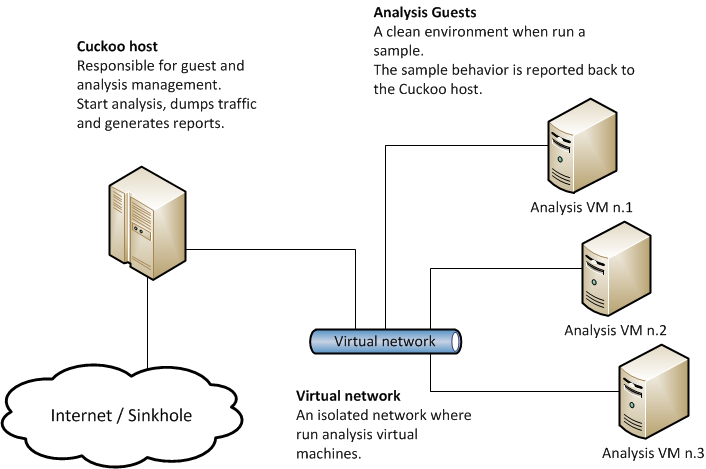
\includegraphics[width=0.8\textwidth]{figures/architecture.png}
  \caption{Official image of sandbox architecture (source \cite{CAPESand75:online})}
  \label{fig:capearchitecture}
\end{figure}

% \todo{if enough time, we should redraw the image and where we may display even result in server and agent.py and capemon.dll, this might be an additional image, more low level}

\subsection{Components}
The sandbox consists internally of several components. They can be seen in figure \ref{fig:capeflow} and their description follows.

\subsubsection*{Scheduler}
This component runs on \emph{host} machine. It checks configured limits and proper setup. It manages machinery modules and starts the new task if there is a pending \emph{guest}. A new task is forwarded to \emph{analysis manager}.

\subsubsection*{Analysis manager}
\emph{Analysis manager} is responsible for the whole flow of a single task. It starts other modules which are part of the analysis and starts/stops the machine through \emph{machinery modules}.

\subsubsection*{Machinary modules}
These modules are used by sandbox to manage virtual machines - start, stop, restore. They are initialized during sandbox startup. Recommended  software for virtual machine management in \emph{CAPEv2} is \emph{KVM}.

\subsubsection*{Guest manager}
This component communicates with the \emph{agent}. It uploads the sample, checks the state of the analysis and the machine, shutdowns the machine in case of timeout.

\subsubsection*{Cape agent}
\emph{Agent} is an HTTP server running inside \emph{guest} machine to report its state and allow sample upload and related actions. It has to start simultaneously with the machine startup (added to the Windows Startup directory).

\subsubsection*{Analyzer}
It is a platform-dependent software running in \emph{guest} machine that controls the flow in the machine. It is started by \emph{agent} and its configuration is provided per analysis. It runs sample using a chosen package (specific for each type of uploaded file). If the package is not provided, it might be determined automatically. After running the target sample, it injects it with \emph{cape monitor}.

\subsubsection*{Cape monitor}
DLL, which is injected into the running sample. It logs any captured behaviour using several techniques like hooking functions, following processes, and PE dumping. It also sends results to the \emph{result server}. \emph{Cape monitor} is maintained in separate repository\footnote{https://github.com/kevoreilly/capemon}.

\subsubsection*{Auxiliary modules}
These are additional modules that run before or during analysis in \emph{guest} machine. An example of such a module is the network traffic sniffer that captures network traffic or a screenshot capture tool.

\subsubsection*{Result server}
It collects the analysis results and stores them. It runs on \emph{host} machine.

\subsubsection*{Processing modules}
Processing consists of the following parts - raw data processing, signature matching, and reporting. The first part transforms the raw output to a readable/searchable format, performs static analysis, and extracts network streams. There is a structured output at the end. The second part is running particular signatures and collecting their results. Signatures are stored in a special repository\footnote{https://github.com/kevoreilly/community}. Their interface accepts the processed structured data and generates results indicating that the current signature matches (true or false) and related data. Signature results are added to the structured output. The final part of the analysis is reporting. In this part, all results are stored in \emph{JSON} report and also in the database (other reporting modules might be added).

The list of raw data processing modules:
\begin{itemize}
  \itemsep0em 
  \item AnalysisInfo - basic information about analysis
  \item BehaviorAnalysis - parses the raw behavioural logs and performs some initial transformations and interpretations, including the complete processes tracing, behavioural summary and process tree
  \item Debug - parses errors and analysis.log generated by the analyzer
  \item Dropped - parses information on the dropped files by malware and dumped by \emph{CAPE}
  \item Memory - executes Volatility analysis on a full memory dump
  \item NetworkAnalysis - parses the PCAP file and extracts some network information, such as DNS traffic, domains, IPs, HTTP requests, IRC and SMTP traffic
  \item ProcMemory - performs analysis of process memory dump
  \item StaticAnalysis - performs static analysis of PE32 files
  \item Strings - extracts strings from the analyzed binary
\end{itemize}

A Signature might isolate some unique behaviour, identify some malware family or type, and spot significant modifications performed in the system. The signature report consists of an identifier, description, severity, category, and other related information.

\subsection{Analysis flow}
A target file upload might be performed using CLI utility of \emph{CAPEv2}, using the Web interface,  Python API or REST API.

If a file is uploaded \emph{CAPEv2} saves it to the database. Multiple options could be configured for each analysis - used package, machine to run on, network setup, timeout, priority, and multiple additional options. We can run only network analysis or only static analysis. The \emph{scheduler} keeps track of pending tasks and runs them. The process of execution is managed by \emph{analysis manager}. In case of running a new analysis, \emph{analysis manager} informs the \emph{result server}. When the analysis is running, the \emph{analyzer, monitor}, configuration and the sample file are uploaded to the \emph{guest} using \emph{agent}. \emph{Agent} starts the \emph{analyzer}, run the sample and injects \emph{monitor} to that. The \emph{analyzer} and \emph{monitor} sends results to the \emph{result server}. After the analysis stops or timeout passes, \emph{analysis manager} stops the machine. The collected analysis results are forwarded to \emph{processing modules}. Results are stored in the chosen formats and saved to the database \cite{CuckooSa10:online}. The whole flow can be seen in figure \ref{fig:capeflow}.

\begin{figure}[h]
  \centering
  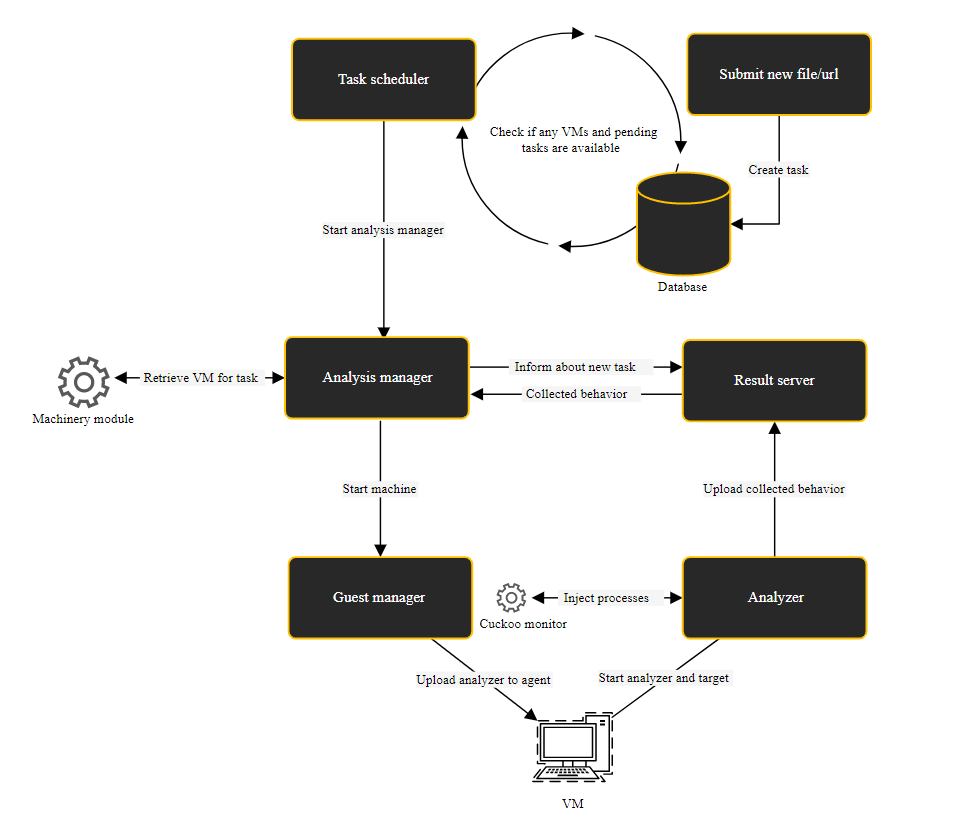
\includegraphics[width=0.8\textwidth]{figures/flow.png}
  \caption{\emph{CAPEv2} components and analysis flow (source \cite{CuckooSa10:online})}
  \label{fig:capeflow}
\end{figure}


\subsection{Network setup options}
\emph{CAPEv2} provides multiple possibilities for \emph{guest} network setup which could be configured per analysis. 

In the case of \emph{None} routing, the machine is isolated. The only connection is the one with the result server. Additionally, there is \emph{Drop} routing when all the traffic is actively dropped (a more aggressive option). 

Other options provide internet connection (in some sense). \emph{Internet} routing is full internet access through specified interface. We can also forward the traffic through another gateway, i.e. \emph{VPN}, \emph{SOCKS5} proxy\footnote{example tool https://github.com/RicoVZ/socks5man} or \emph{Tor}\footnote{https://www.torproject.org/}. Last option is to use network simulation like \emph{INetSim}\footnote{https://www.inetsim.org/}.

\subsection{Other features}
One of the crucial features of \emph{CAPEv2} is the debugger, so we can also perform non-interactive dynamic code analysis. It allows dynamic anti-evasion bypasses such as \emph{Guloader, Ursnif} or \emph{Zloader} uses.

\emph{CAPE} means \emph{Config And Payload Extraction}. The main motivation behind its creation was malware payload extraction, for which it uses techniques like Process injection, Decompression of executable modules in memory or extraction of executable modules. \emph{CAPEv2} automatically creates a process dump for each process that effectively detects the basic packers.

It can detect various malware families such as Emotet, QakBot, Dridex, and many others. It also uses Yara rules.

\subsection{Produced data}
The whole ouput of \emph{CAPEv2} is listed in the table \ref{tab:sandbox-out}.


\subsubsection{Report}
As we stated in the thesis introduction, our goal is to use \emph{behavioural} features and \emph{signatures} from \emph{JSON} reports.  The most comprehensive report produced by \emph{CAPEv2} is in \emph{JSON} format. We will use this format as direct input for our model. Let us define this format \footnote{documentation https://www.json.org/json-en.html} and the content of the report.

JSON (JavaScript Object Notation) is the most frequently used lightweight data interchange format. It consists of two essential structures - \emph{collections of key-value pairs} (sometimes called \emph{objects}) and \emph{ordered lists}. 

\emph{Object} is an unordered list of \emph{key-value} pairs, curly brackets surround it, pairs are coma-separated, and a colon separates keys from values. \emph{Keys} have to be double-quoted Unicode strings. \emph{Values} might be strings, numbers, objects, arrays, boolean or null. \emph{Lists} are surrounded by square brackets and contain comma-separated values.

Usually, a single \emph{.json} file contains one object, but there are also cases where a list of objects is presented.

The \emph{CAPEv2} report usually has tens of megabytes but sometimes even gigabytes. Complete schema (list of attributes) of report is in \ref{tab:report}. In the thesis attachment, we can see an example of a real log (\ref{app:attach}). In the modelling part, we will concentrate on \emph{signatures} and the \emph{behaviour} parts (its structure is described in figure \ref{tab:behavioral}).


\section{Prior arts}
Below we list relevant publications where the authors applied a machine learning algorithm to the data produced by malware analysis tools.
\subsubsection*{Static features}
\begin{itemize}
  \itemsep0em 
  \item Strings - \cite{Lee2011}
  \item N-grams (analysis of byte subsequences of length $N$ from the original binary) - \cite{Fuyong2017}
  \item Entropy of the malware file - \cite{Wojnowicz2018}
  \item Statically extracted API function calls - \cite{Ahmadi2016}
\end{itemize}

\subsubsection*{Dynamic features}
\begin{itemize}
  \itemsep0em 
  \item Registry - \cite{Ghiasi2015}
  \item CPU instruction traces - \cite{Carlin2017}
  \item Network traffic - \cite{Boukhtouta2015}
  \item API call traces -  \cite{Galal2015}
\end{itemize}

Other related resources might be \cite{Singh2020, Sethi2019, Abdessadki2019, Gibert2020}.

%%------------------------------------------
% Let us summarize basics of malware interaction with windows OS (main source \cite{Sikorski2012}). nice to have chapter ANALYZING MALICIOUS
% WINDOWS PROGRAMS
% Types, Families
% https://en.wikipedia.org/wiki/Malware
% Find in books!
% https://www.sciencedirect.com/science/article/pii/S1084804519303868 - good overview and taxonomy of malware


% \todo{describe part one goal - We involve more theory and prior work research, in following chapters we discuss our case.}
% In the first part of this thesis we focus the comprehensive theory which is needed to absorb in order to interpret results. Not everything is disassembled in detail we go only there where we find something useful for our thesis. This is really based on experience so if the reader is interested only in results used formalism and notation in theory part are important only.

% \todo{Summarise what we know from previous sections \todo{especially from analysis part, where we should summarise what usual program is doing in the computer and what we can observe (and what we can get from cuckoo monitor)} and go to the most concetrated information about run of program - we should end at the things which are in summary part of json log, but we can have more variants}



% Last remarkable not is many times analyzed statistical assumption
% My
% Data quality, bias, antisandbox detection... where to find samples? (we should definitely mention motivation why we are collecting our own data), public data (this is quite risky to publish in general), everything is fast (zero days), Are those anomalies or malicious?, Imbalanced data sets, encryption everywhere - what to trust..., cryptocurrencies, iot, cloud

% \todo{add some motivation example or latest results... - known malware attacks..}

% Philosophy could be walking around risk management, probability of risk and resulting damage... Maybe more examples of situations where we know how much it cost (Cambridge analytica, ransomware...)
% Maybe something about truth and its protection in the world of lies and fake news
% Confidentiality, integrity and availability

% Use found books or post-hoc go through some articles and formulate the motivation part...



% Nice to have
% https://github.com/kevoreilly/CAPEv2/blob/master/changelog.md
% http://docplayer.net/62887099-Cuckoo-malware-analysis.html
% https://cuckoo-monitor.readthedocs.io/en/latest/hooks.html, more comprehensive description of cape monitor
% Processing modules

% existing solutions and results...
% find basics in books

% api hooking, dumping import reconstruction debugging static parsing - https://www.youtube.com/watch?v=qEwBGGgWgOM

% to appendix we can add also web interface of cuckoo
% \section{Prior}
% works about malware analysis
% works that collected data for machine learning purposes
% Mandlik, Stiborek, everybody who used cuckoo or other sandbox data (reference for what and their results)

% file:///C:/Users/domia/Downloads/Imad-Saiida-IJCNIS-V11-N6-1.pdf
% https://web.archive.org/web/20160418151823/http://www.ijarcsse.com/docs/papers/Volume_3/4_April2013/V3I4-0371.pdf
% https://reader.elsevier.com/reader/sd/pii/S1383762120301442?token=81F1AB06FF0FE40D1B7745234269280FCF2CB0979140E84DB35D6E04A2C622FE6EDA2DE4DA0630E1D73044E3D84A722F&originRegion=eu-west-1&originCreation=20210401090943
% https://iopscience.iop.org/article/10.1088/1742-6596/1140/1/012042/pdf
% file:///C:/Users/domia/Downloads/JCIT4024PPL.pdf
% https://dl.acm.org/doi/abs/10.1145/2046614.2046618?casa_token=MXpfHiylCZcAAAAA:szRMPWfKXTl4wxP2-h32eknCg5dzM2t7RxGjywiJDksmT5FqcUY7pPrIBZchv26HUe3Lwubu5Hru

% file:///C:/Users/domia/Downloads/088851962.pdf

% mention signatures
% usual format which are produced by sandbox and what we can find there
% Reference even docs - no problem, not only books and papers
% Conclusion should be that those data are complicated and their structure also keep some information (order, structure...), that is why we want to focus on structured data and especially json.
% size...


% TODO - nice-to-have
% memory forensics


% If I have to add something - https://publications.sba-research.org/publications/malware_survey.pdf



% mention especially parts which gives more information about the run (mutexes, files, api calls,.. - to be able to reference from data chapter)

% - Summary of potential sorces of metadata
% ○ Abuse.ch - https://bazaar.abuse.ch/api/#api_key
% ○ VirusTotal - https://developers.virustotal.com/v3.0/reference#file-info
% ○ Metadefender - https://onlinehelp.opswat.com/mdcloud/3.1_Retrieving_scan_reports_using_a_data_hash.html
% - Interesting



% Previous connection
% - Nothing before
% Way through this chapter
% - Malware definition and types
% - Malware analysis
% - Challenges
% - Data - input, output...
% - prior
% Next connection
% - We are interested in modeling the data using modern approaches, we know that the data are often structured somehow and that is what we will solve

% - GOALS
%   - Run several instances of CapeV2 sandbox and solve their orchestration for this experiment
%   - Capture behavior of selected malware samples in CapeV2 sandbox and store results
% - Theory part - types, conditions, bias, Malware types, signatures....
% - Sandboxing
% - Previous experiments
% - Our goal in this part
% - Data collection for ML purposes in general


% https://www.groundai.com/project/machine-learning-in-cyber-security-problems-challenges-and-data-sets/1

% https://www.readitquik.com/articles/security-2/cybersecurity-challenges-that-need-to-be-on-your-radar-right-now/